%        File: assg2.tex
%     Created: Fri Oct 08 05:00 PM 2010 P
% Last Change: Fri Oct 08 05:00 PM 2010 P
%
\documentclass[a4paper,12pt]{article}
\usepackage{amsmath}
\usepackage{graphicx}
\begin{document}
\title{Homework 2}
\author{Matt Forbes}
\date{October 12, 2010}
\maketitle
\section*{Problem 3.1}
\subsection*{a\()\)}
\begin{alignat*}{6}
  \min \quad -2x_1& - 3x_2& {}& {}& {}& \\
  \text{s. t.} \quad \quad x_1& + x_2& + x_3& {}& = 4 \\
  x_1& - 2x_2& {}& + x_4& = 1 \\
  {}& \mathbf{x} \ge 0
\end{alignat*}
\subsection*{b\()\)}
\begin{center}
  \begin{tabular}{| c | c c c c |}
    \hline
    0 & -2 & -3 & 0 & 0 \\
    \hline
    4 & 1 & 1 & 1 & 0 \\
    1 & 1 & -2 & 0 & 1 \\
    \hline
  \end{tabular}
\end{center}
\subsection*{c\()\)}
\begin{center}
  \begin{tabular}{| c | c c c c |}
    \hline
    2 & 0 & -7 & 0 & 2 \\
    \hline
    3 & 0 & 3 & 1 & -1 \\
    1 & 1 & -2 & 0 & 1 \\
    \hline
  \end{tabular}
\end{center}
\begin{center}
  \begin{tabular}{| c | c c c c |}
    \hline
    9 & 0 & 0 & \(\frac{7}{3}\) & \(-\frac{1}{3}\) \\
    \hline
    1 & 0 & 1 & \(\frac{1}{3}\) & \(-\frac{1}{3}\) \\
    3 & 1 & 0 & \(\frac{2}{3}\) & \(\frac{1}{3}\) \\
    \hline
  \end{tabular}
\end{center}
\begin{center}
  \begin{tabular}{| c | c c c c |}
    \hline
    12 & 1 & 0 & 3 & 0 \\
    \hline
    4 & 1 & 1 & 1 & 0 \\
    9 & 3 & 0 & 2 & 1 \\
    \hline
  \end{tabular}
\end{center}
{\bf optimal form: x = \((0, 4, 0, 9)^T\)}
\subsection*{d\()\)}
\begin{center}
  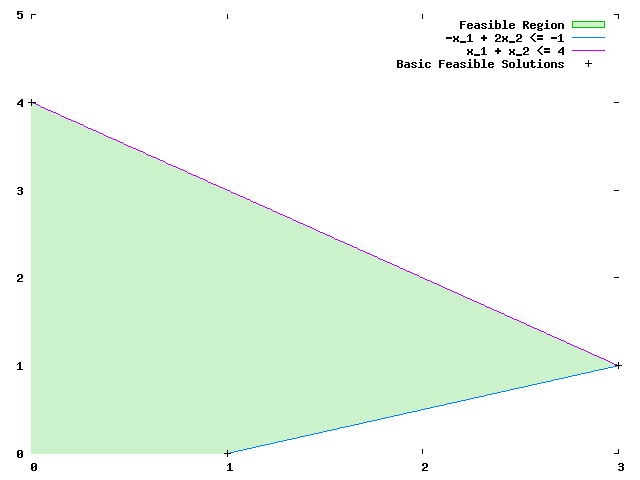
\includegraphics[width=10cm, height=10cm, keepaspectratio=true]{31.png}
\end{center}
\section*{Problem 3.2}
\subsection*{a\()\)}
\begin{alignat*}{5}
  \min \quad -2x_1& + x_2 \\
  \text{s.t} \quad \quad x_1& + 2x_2& + x_3& {}& = 10 \\
  -x_1& + x_2& {}& - x_4& = 5 \\
  {}& \mathbf{x} \ge 0
\end{alignat*}
\subsection*{b\()\)}
If moving from original problem to standard form: \\
\begin{itemize}
  \item The feasible point is of the form \( (x_1 \quad x_2)^T \)
  \item A point for the standard form needs an \( x_3 \text{ and } x_4 \), which
    are equal to \(10 - x_1 - 2x_2\) and \(-x_1 + x_2 - 5\) respectively.
  \item So this solution in the standard form would be: \\
    \begin{center}
      \(\left(
      \begin{array}{c}
	x_1\\ x_2\\ 10 - x_1 - 2x_2\\ -x_1 + x_2 - 5
      \end{array}
      \right)\)
    \end{center}
\end{itemize}
If moving from standard form to original problem:
\begin{itemize}
  \item The feasible point is \( (x_1 \quad x_2 \quad x_3 \quad x_4)^T \)
  \item Only \(x_1\) and \(x_2\) are needed for original form, so the solution would be: \\
    \begin{center}
      \(\left(
      \begin{array}{c}
        x_1 \\ x_2
      \end{array}
      \right)\)
    \end{center}
\end{itemize}
\subsection*{c\()\)}
Both programs are optimizing the same function with the same constraints. Therefore, if a minimum is
found for one program, it is the minimum for the other.
\subsection*{d\()\)}
Same reasoning as part c. They are the same problem, just formatted differently. There cannot be different
solutions.
\subsection*{e\()\)}
You're kidding right? They are the same problem.
\section*{Problem 3.3}
  \begin{center}
    \begin{tabular}{| c | c | c | c | c | c |}
      \hline
      & a & b & c & d & e \\ \hline
      i & \( \ge 0 \) & \( \ge 0 \) & c & d & \( \ge 0 \) \\ \hline
      ii & \( \ge 0 \) & \( < 0\) & \(< 0\) & \(< 0\) & e  \\ \hline
      iii & \( < 0\) & b & \(\ge 0\) & d & e \\ \hline
      iv & \(\ge 0\) & \(=0\) & c & d & \(=0\)\\
      \hline
    \end{tabular}
  \end{center}
\section*{Problem 3.6}
  \begin{alignat*}{7}
    \min \quad 2x_1& + x_2& - 4x_3& {}& {}& {}& \\
    \text{s.t.} \quad 3x_1& - 2x_2& + 2x_3& + x_4& {}& {}& = 25 \\
    -x_1& - x_2&  + 2x_3& {}& + x_5& {}& = 20 \\
    -x_1& - x_2& + x_3& {}& {}& + x_6& = 5 \\
    {}& \mathbf{x} \ge 0
  \end {alignat*}
  \begin{center}
    \begin{tabular}{| c | c  c  c  c  c  c |}
      \hline
      0 & 2 & 1 & -4 & 0 & 0 & 0 \\
      \hline
      25 & 3 & -1 & 2 & 1 & 0 & 0 \\
      20 & -1 & -1 & 2 & 0 & 1 & 0 \\
      5 & -1 & -1 & 1 & 0 & 0 & 1 \\
      \hline
    \end{tabular}
  \end{center}
  \begin{center}
    \begin{tabular}{| c | c  c  c  c  c  c |}
      \hline
      20 & -2 & -3 & 0 & 0 & 0 & 4 \\
      \hline
      15 & 5 & 1 & 0 & 1 & 0 & 4 \\
      10 & 1 & 1 & 0 & 0 & 1 & -2 \\
      5 & -1 & -1 & 1 & 0 & 0 & 1 \\
      \hline
    \end{tabular}
  \end{center}
  \begin{center}
    \begin{tabular}{| c | c  c  c  c  c  c |}
      \hline
      50 & 7 & 0 & 0 & 0 & 3 & -2 \\
      \hline\
      5 & 2 & 0 & 0 & 1 & -1 & 0 \\
      10 & 3 & 1 & 0 & 0 & 1 & -2 \\
      15 & 2 & 0 & 1 & 0 & 1 & -1 \\
      \hline
    \end{tabular}
  \end{center}
 This problem is unbounded and therefore has no finite optimal solution.
\section*{Problem 3.7}
  \subsection*{a\()\)}
     \begin{center}  
       \begin{tabular}{| c | c c c c c |}
         \hline
         0 & 2 & -1 & 0 & 3 & 0 \\
         \hline
         10 & 1 & 1 & 0 & 1 & 1 \\
         6 & 3 & -1 & 1 & -2 & 0 \\
         \hline
      \end{tabular}
    \end{center}
  \subsection*{b\()\)}
    Basic sequence \(S = \{ 5, 1\}\)
  \subsection*{c\()\)}
  Basic feasible solution \(\mathbf{x} = 
    \left( 
    \begin{array}{c}
      0 \\ 0 \\ 6 \\ 0 \\ 10
    \end{array}
    \right)
    \)
  \subsection*{d\()\)}
    Solving 1st constraint for \(x_2\): \(x_2 = 10 - x_1 - x_4 - x_5\) \\
    Replacing \(x_2\) in objective function: \(-10 + 3x_1 + 4x_4 + x_5\) \\
    Replacing \(x_2\) in 2nd constraint: \(4x_1 + x_3 - x_4 + x_5 = 16\) \\
    Which produces a new LP problem:
    \begin{alignat*}{6}
      \min \quad 3x_1& {}& {}& + 4x_4& + x_5& - 10 \\
      \text{s.t} \quad \quad x_1& + 2x_2& + x_3& + x_4& {}& = 10\\
      x_1& {}& + x_3& - x_4& + x_5& = 16 \\
    \end{alignat*}
    Which has a simplex tableau of:
    \begin{center}
      \begin{tabular}{| c | c c c c c |}
	\hline
	-10 & 3 & 0 & 0 & 4 & 1 \\
	\hline
	10 & 1 & 2 & 1 & 1 & 0 \\
	16 & 4 & 0 & 1 & -1 & 1 \\
	\hline
      \end{tabular}
    \end{center}
    Likewise, \\
    Pivoting in the 2nd column of the tableau from a) results in the same form as above. \\
    \begin{center}
      \begin{tabular}{| c | c c c c c |}
	\hline
	-10 & 3 & 0 & 0 & 4 & 1 \\
	\hline
	10 & 1 & 2 & 1 & 1 & 0 \\
	16 & 4 & 0 & 1 & -1 & 1 \\
	\hline
      \end{tabular}
    \end{center}

\section*{Problem 3.10}
\section*{Problem 3.11}
\section*{Problem 3.22}

\end{document}


